\section{Lecture 12 (22 V 2019)}
\begin{figure}[H]
    \centering
    \caption{Replica of prof. Niwiński's drawing}
    
\includegraphics[scale=0.1]{content/graphics/game25.png}
\end{figure}
\begin{figure}[H]
    \centering
    \caption{Rock-paper-scissors does not have an equilibrium}
    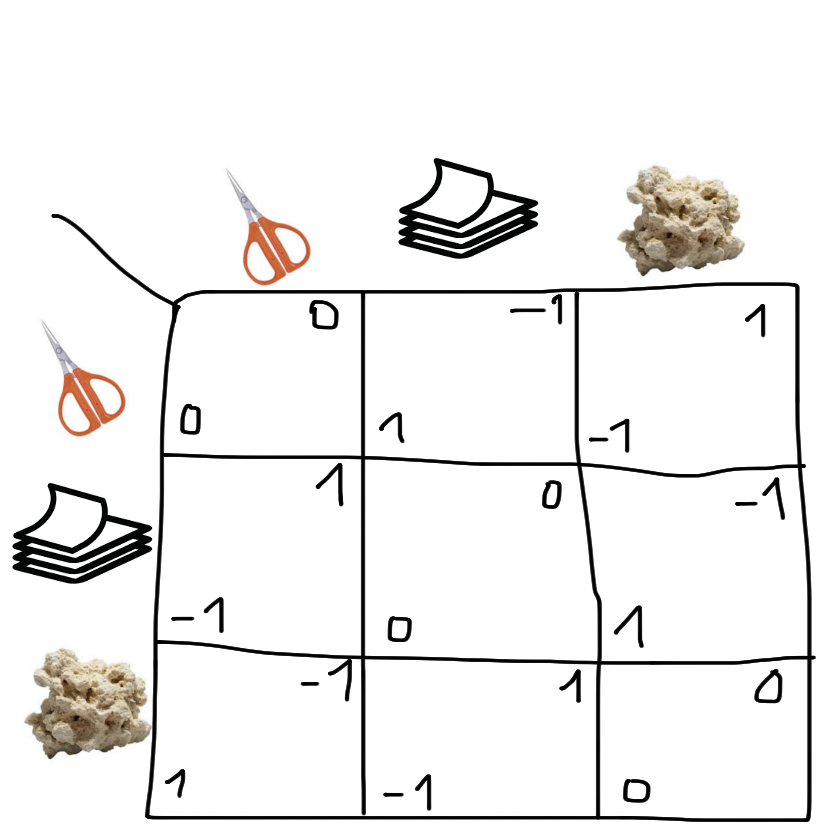
\includegraphics[scale=0.1]{content/graphics/game26.png}
\end{figure}

\subsection*{Nash equilibrium}
Let $(S, f)$ be a game with $n$ players, where $S_i$ is the strategy set for player
$i$, $S = S_1 \times S_2 \times ... \times S_n$ is the set of strategy profiles
\footnote{
a vector of exactly one strategy for each player, fully determining the play
}
and $f(x) = (f_1(x), ..., f_n(x))$ is its payoff function evaluated at $x \in S$.
Let $x_i$ be a strategy for player $i$ and let $x_{-i}$ be a strategy profile
for all players other than $i$. When each player $i \in \{1, ..., n\}$ chooses
strategy $x_i$ resulting in strategy profile $x = (x_1, ..., x_n)$ then player $i$
obtains payoff $f_i(x)$. Note that the payoff depends on the strategy profile
chosen, i.e. on the strategy chosen by player $i$ as well as strategies chosen by
others. A strategy profile $x^{*} \in S$ is a Nash equilibrium if no unilateral
deviation in strategy by any single player is profitable for that player, that is
$\forall_{i, x_i \in S_i} f_i(x_i^{*}, x_{-i}^{*}) \geq f_i(x_i, x_{-i}^{*})$.